%-----Main FIle------
%For Detail check out - http://firesofmay.blogspot.com/2011/10/latex-project-report-template
%CHANGE THESE Settings ONLY IF YOU KNOW WHAT YOU DOING

\documentclass[12pt,a4paper]{article}

%adjust your page margins here
\usepackage[top=0.70in, bottom=0.70in, left=0.8in,right=0.80in]{geometry} % setting the page alignment with this package
\usepackage[pdftex]{graphicx} %for embedding images
%\usepackage[hyphens]{url} %for proper url entries
\usepackage[dvips, bookmarks, colorlinks=false]{hyperref} %for creating links in the pdf version and other additional pdf attributes, no effect on the printed document
\usepackage[final]{pdfpages} %for embedding another pdf, remove if not required
\usepackage{float} %used for figure placement with H as a parameter
%\usepackage[hyphens]{url}
%\usepackage{hyperref}
\usepackage{pslatex} % for times new roman, old package, but works
\usepackage{array} % for making text bold in table


%For inserting Python Code
\usepackage{listings}
\usepackage{color}
 
\definecolor{dkgreen}{rgb}{0,0.6,0}
\definecolor{gray}{rgb}{0.5,0.5,0.5}
\definecolor{mauve}{rgb}{0.58,0,0.82}
 
\lstset{ %
  language=Java,                % the language of the code
  basicstyle=\footnotesize,           % the size of the fonts that are used for the code
  numbers=left,                   % where to put the line-numbers
  numberstyle=\tiny\color{gray},  % the style that is used for the line-numbers
  stepnumber=1,                   % each line is numbered
  numbersep=5pt,                  % how far the line-numbers are from the code
  backgroundcolor=\color{white},      % choose the background color. You must add \usepackage{color}
  showspaces=false,               % show spaces adding particular underscores
  showstringspaces=false,         % underline spaces within strings
  showtabs=false,                 % show tabs within strings adding particular underscores
  frame=single,                   % adds a frame around the code
  rulecolor=\color{black},        % if not set, the frame-color may be changed on line-breaks within not-black text (e.g. commens (green here))
  tabsize=2,                      % sets default tabsize to 2 spaces
  captionpos=b,                   % sets the caption-position to bottom
  breaklines=true,                % sets automatic line breaking
  breakatwhitespace=false,        % sets if automatic breaks should only happen at whitespace
  title=\lstname,                   % show the filename of files included with \lstinputlisting;
                                  % also try caption instead of title
  keywordstyle=\color{blue},          % keyword style
  commentstyle=\color{dkgreen},       % comment style
  stringstyle=\color{mauve},         % string literal style
  escapeinside={\%*}{*)},            % if you want to add a comment within your code
  morekeywords={*,...}               % if you want to add more keywords to the set
}

%%%%For inserting Python Code Over



%For the header and footer
\usepackage{fancyhdr}
\fancypagestyle{plain}{%
%\fancyhf{} % clear all header and footer fields
\fancyfoot[L]{} % except the center
\fancyfoot[R]{\thepage}
\renewcommand{\headrulewidth}{0.4pt}
\renewcommand{\footrulewidth}{0.4pt}
}



\fancyfoot[LO,LE]{}
\cfoot{}
\fancyfoot[RO, RE]{\thepage}
\renewcommand{\headrulewidth}{0.4pt}
\renewcommand{\footrulewidth}{0.4pt}
%For the header and footer Over

% Altering the Index Page Title
%\renewcommand{\contentsname}{\begin{center}\textsc{University Of Pune \\2011 - 2012}\\[1cm]Index\end{center}} 


%GLOBAL SETTINGS OVER, DOCUMENT BEGINS
\begin{document}



%FROM HERE YOUR PAGES START GETTING ADDED

% includes the cover page
\begin{titlepage}
 \newcommand{\HRule}{\rule{\linewidth}{0.5mm}}
 \center
 
 
 \textsc{\LARGE Concordia University}\\[1.5cm]
 \begin{figure}[h]
 \centering
 
\includegraphics[width=12cm]{images/cover/concordia}
 \end{figure}

 \textsc{\large INSE 6140}\\[0.5cm]
 \textsc{\large Middleware and Application Security}
 
 
 \HRule \\[0.4cm]
 {
  \Huge \bfseries Puzzlr: a secure decentralized image sharing mobile application.
 }
 \HRule \\[1.5cm]
 
 
 \begin{minipage}{1\textwidth}
  \begin{flushleft}
   \center Aniss \textsc{Chohra} (40001217)
  \end{flushleft}
  \begin{flushleft}
   \center Quentin \textsc{Le Sceller} (40002477)
  \end{flushleft}


 \end{minipage}
 ~
 \newline
 \newline
 
 
 \begin{minipage}{1\textwidth}
 
  \begin{flushleft}
   \emph{Submitted to:} \\
   Professor Makan \textsc{Pourzandi}
  \end{flushleft}

 \end{minipage}\\[4cm]
 
 
 {\large \today}\\[3cm]
 
 \vfill


\end{titlepage}
 
\newpage
\pagestyle{fancy}


\pagenumbering{arabic}


%TABLE OF CONTENTS AND LIST OF FIGURES ARE AUTOMATICALLY ADDED BY FOLLOWING COMMANDS
%ADD FIGURE OF TABLES IF YOU NEED TO, CHECK DOCUMENTATION
%numbering before main content starts


%To reset the Header & Footer for TOC and LOF
%\pagestyle{empty}
%\addtocontents{toc}{\protect\thispagestyle{empty}}
\tableofcontents % adds Index Page
\newpage
%\pagestyle{empty}

%\addtocontents{lof}{\protect\thispagestyle{empty}}
\listoffigures % adds List of Figures
\newpage

%And reset back the settings we choose for Header and Footer
 %reset numbering to normal for the main content

\section{Abstract}
  \paragraph{}
\section{Introduction}
  \paragraph{}
    
\section{Related work}
  \paragraph{}
\section{Threat model}
  \paragraph{}
\section{General Architecture}
    \paragraph{}
    In this part, we present a global overview over Puzzlr's architecture. We used a semi-decentralized scheme where in each session, there are three major participating parties (figure 1).
      \begin{figure}[H]   
	\centering
	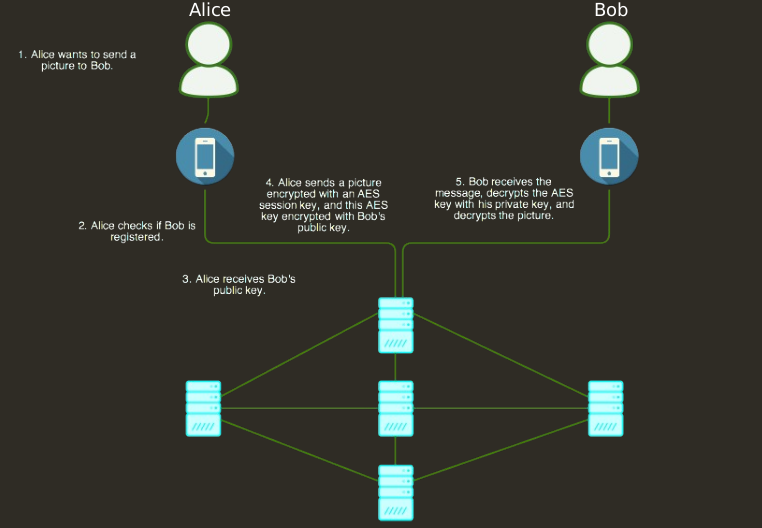
\includegraphics[width=16cm]{images/architecture/architecture}
	\caption{Puzzlr: General Architecture.}
	\label{Figure 1}
      \end{figure}
      \subsection{Registration Phase}
      
	\paragraph{}
	  When two clients want to register on the application, say Alice and Bob, they will both generate an RSA key pair. Their respective public keys are then sent to the server to be stored on the database (figure 2).
	  
	  \begin{figure}[H]  
	    \centering
	    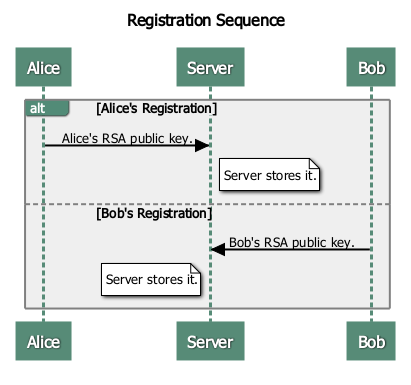
\includegraphics[width=8cm]{images/architecture/registrationsequence}
	    \caption{Registration phase Sequence Diagram.}
	  \end{figure}
	  \subsection{Retrieval of Other Correspondant's Public key}
	  \paragraph{}
	  
	    If let's say Alice wants to send a message to Bob, she will first have to find his corresponding public key. To achieve that, she will send a request to the server which will query the database to check if Alice and Bob are both registered first, if that is the case, the server will then send Bob's public key to Alice (figure 3).
	    
	    \begin{figure}[H]
	      \centering
	      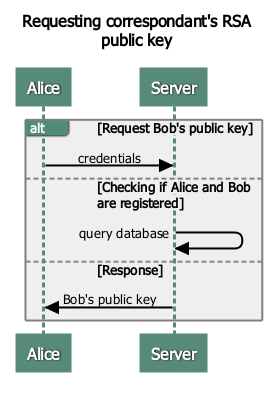
\includegraphics[width=8cm]{images/architecture/requestingcorrespondant'sRSApublickey}
	      \caption{Requesting Correspondant's RSA public key Sequence Diagram.}
	    \end{figure}
	    
	    
	    \subsection{Picture Sending and Receival}
	    \paragraph{}
	    
	    After retrieving Bob's public key from the server, Alice will now do the following steps (figure 4):
	    
	    \begin{itemize}
	     \item Choose a picture to send.
	     \item Generate a session key (AES) and a MAC key.
	     \item Generate a random IV.
	     \item Encrypt the AES key, the MAC key, and her username using Bob's public key (message 1).
	     \item Encrypt the picture that she picked with the AES key and the IV (message 2).
	     \item Generate a MAC tag using the MAC key on the second message (message 2) and the IV (message 3).
	     \item Send the three messages to the server concatenated (message 1 + message 2 + message 3).
	    \end{itemize}
	    
	    \begin{figure}[H]
	    
	      \centering
	      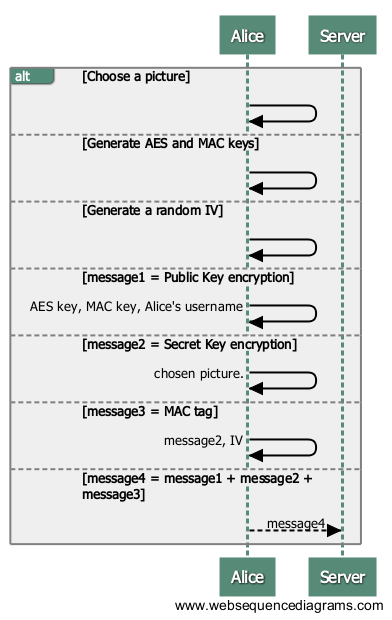
\includegraphics[width=8cm]{images/architecture/picture_sending}
	      \caption{Picture Sending}
	     
	    \end{figure}
	    
	    \paragraph{}
	      On the other hand, when the server receives Alice's message, it will forward this message to Bob. Bob will receive the message and (figure 5):
	      \begin{itemize}
	       \item Recovers the AES key, MAC key, and Alice's username using his private key.
	       \item Checks if the MAC tag received is valid by computing a new one on the received AES ciphertext and the IV, and then compares between them.
	       \item Finally, recovers the picture using the recovered AES key and the IV.
	      \end{itemize}

	    \begin{figure}[H]
	    
	      \centering
	      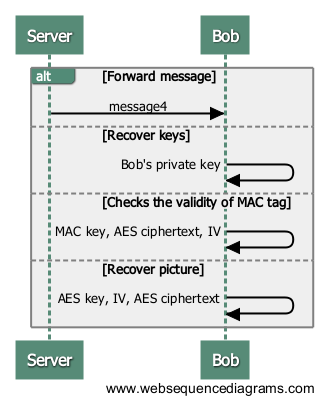
\includegraphics[width=8cm]{images/architecture/receive}
	      \caption{Picture Receival}
	     
	    \end{figure}

	    
	    
	    




	  
      
      
     
      


	
  
\section{Cryptography}
  \subsection{Client-Server Communication}
  \subsection{Password Storage}
  \subsection{Data Encryption}
\section{Implementations}
  \subsection{Server side}
  \subsection{Client side}
    \subsubsection{Android (Aniss)}
      \paragraph{}
	The Android version is written in Java Programming Language alongside with some parts in XML (the Graphical User Interface). In this project we used Android Studio as an Integrated Developpement Environment (IDE). The application is compatible with almost all versions of Android.
	\paragraph{}
	The source code is open source and is available at this link along with the installation details:
	\paragraph{}
	\color{blue}\underline{https://github.com/aniss05/Puzzlr2}\color{black} 
	  
    \subsubsection{IOS}
\section{Discussion and Future Work}
\section{Conclusion}
\begin{thebibliography}{60}
 \bibitem{}
\end{thebibliography}




\end{document}
